\documentclass{article}

\usepackage{fancyhdr}
\usepackage{extramarks}
\usepackage{amsmath}
\usepackage{amsthm}
\usepackage{amsfonts}
\usepackage{tikz}
\usepackage[plain]{algorithm}
\usepackage{algpseudocode}
\usepackage{placeins}
\usepackage{tcolorbox}

\usetikzlibrary{automata,positioning}

%
% Basic Document Settings
%

\topmargin=-0.45in
\evensidemargin=0in
\oddsidemargin=0in
\textwidth=6.5in
\textheight=9.0in
\headsep=0.25in

\linespread{1.1}

\pagestyle{fancy}
\lhead{\hmwkAuthorName}
\chead{\hmwkClass\: \hmwkTitle}
\rhead{\firstxmark}
\lfoot{\lastxmark}
\cfoot{\thepage}

\renewcommand\headrulewidth{0.4pt}
\renewcommand\footrulewidth{0.4pt}

\setlength\parindent{0pt}

\newtheorem{subproblem}{Subproblem}

\tcbuselibrary{theorems}

\newtcbtheorem[number within=section]{mytheo}{Definition}%
{colback=blue!5,colframe=blue!35!black,fonttitle=\bfseries}{th}

%
% Create Problem Sections
%

\newcommand{\enterProblemHeader}[1]{
    \nobreak\extramarks{}{Problem \arabic{#1} continued on next page\ldots}\nobreak{}
    \nobreak\extramarks{Problem \arabic{#1} (continued)}{Problem \arabic{#1} continued on next page\ldots}\nobreak{}
}

\newcommand{\exitProblemHeader}[1]{
    \nobreak\extramarks{Problem \arabic{#1} (continued)}{Problem \arabic{#1} continued on next page\ldots}\nobreak{}
    \stepcounter{#1}
    \nobreak\extramarks{Problem \arabic{#1}}{}\nobreak{}
}

\setcounter{secnumdepth}{0}
\newcounter{partCounter}
\newcounter{homeworkProblemCounter}
\setcounter{homeworkProblemCounter}{1}
\nobreak\extramarks{Problem \arabic{homeworkProblemCounter}}{}\nobreak{}

%
% Homework Problem Environment
%
% This environment takes an optional argument. When given, it will adjust the
% problem counter. This is useful for when the problems given for your
% assignment aren't sequential. See the last 3 problems of this template for an
% example.
%
\newenvironment{homeworkProblem}[1][-1]{
    \ifnum#1>0
        \setcounter{homeworkProblemCounter}{#1}
    \fi
    \section{Problem \arabic{homeworkProblemCounter}}
    \setcounter{partCounter}{1}
    \enterProblemHeader{homeworkProblemCounter}
}{
    \exitProblemHeader{homeworkProblemCounter}
}

%
% Homework Details
%   - Title
%   - Due date
%   - Class
%   - Section/Time
%   - Instructor
%   - Author
%

\newcommand{\hmwkTitle}{Past Paper May 2022}
\newcommand{\hmwkDueDate}{May 5, 2023}
\newcommand{\hmwkClass}{ASR}
\newcommand{\hmwkAuthorName}{\textbf{Patrick Tourniaire}}

%
% Title Page
%

\title{
    \vspace{2in}
    \textmd{\textbf{\hmwkClass:\ \hmwkTitle}}\\
    \normalsize\vspace{0.1in}\small{Completed\ on\ \hmwkDueDate}\\
    \vspace{3in}
}

\author{\hmwkAuthorName}
\date{}

\renewcommand{\part}[1]{\textbf{\large Part \Alph{partCounter}}\stepcounter{partCounter}\\}

%
% Various Helper Commands
%

% Useful for algorithms
\newcommand{\alg}[1]{\textsc{\bfseries \footnotesize #1}}

% For derivatives
\newcommand{\deriv}[1]{\frac{\mathrm{d}}{\mathrm{d}x} (#1)}

% For partial derivatives
\newcommand{\pderiv}[2]{\frac{\partial}{\partial #1} (#2)}

% Integral dx
\newcommand{\dx}{\mathrm{d}x}

% Alias for the Solution section header
\newcommand{\solution}{\textbf{\large Solution}}

% Probability commands: Expectation, Variance, Covariance, Bias
\newcommand{\E}{\mathrm{E}}
\newcommand{\Var}{\mathrm{Var}}
\newcommand{\Cov}{\mathrm{Cov}}
\newcommand{\Bias}{\mathrm{Bias}}

\begin{document}

\maketitle

\pagebreak


% Problem 1
\begin{homeworkProblem}
    
    % Sub-problem 1
    \begin{subproblem}
        What is the difference, if any, between pitch and fundamental frequency?
    \end{subproblem}

    \textbf{Answer}

    The fundemental frequency is closely related to pitch, which is defined as our perception of fundemental frequency. That is, the $F0$
    describes the actual physical phenomenon, whereas pitch describes how our ears and brains intrepret the signal, in terms of periodicity.


    % Sub-problem 2
    \begin{subproblem}
        When we hear the high voice of children, is it because of their shorter
        vocal tract, their shorter vocal fold, or both? Why?
    \end{subproblem}

    \textbf{Answer}

    When we hear the high-pitched voices of children, it is mainly due to the shorter length of their vocal tract, rather than the lenght of
    their vocal folds. The pitch of a voice is determined by the frequency of the vibrations produced by the vocal folds. When the vocal
    folds vibrate at a higher frequency, the resulting sound has a higher pitch. However, the vocal tract, which includes the mouth, throat,
    and nasal cavity, also plays a significant role in shaping the sound produced by the vocal folds.

    In children, the vocal tract is shorter and narrower than in adults, which results in a higher resonance frequency. This means that when
    the vocal folds vibrate, the resulting sound waves are amplified at a higher frequency, resulting in a higher-pitched voice. As children
    grow and their vocal tract elongates, their voices gradually deepen and become lower in pitch.
    
    So, to sum up, the high-pitched voices of children are primarily due to the shorter length of their vocal tract, which amplifies the
    higher-frequency vibrations produced by their vocal folds.


    % Sub-problem 3
    \begin{subproblem}
        In the ideal speech production model described in class, what is the
        connection, if any, between formants and fundamental frequency?
    \end{subproblem}

    \textbf{Answer}

    The fundemental frequency is the first frequency component of the glottal pulse, whereas formants are the resonance frequencies of the vocal
    tract. Which leads to the production and perception of certain phones, particularly vowels.

    
    % Sub-problem 4
    \begin{subproblem}
        Could we infer fundamental frequency from log Mel spectrograms? If
        so, how?
    \end{subproblem}

    \textbf{Answer}

    Yes, it is possible to infer the fundemental frequency (also know as $F0$ or pitch) from log Mel spectrograms is to use a technique called the
    autocorrelation method. The basic idea behind this method is to calculate the correlation between the spectogram and a delayed version of itself,
    and then identify the delay that results in the highest correlation. This delay corresponds to the period of the fundemental frequency, which can
    be used to calculate the $F0$.

    Another approach is to use a DNN based method to directly estimate $F0$ from the log Mel spectogram. This involves training a NN on a large dataset
    of audio recordings and their corresponding $F0$ values, so that the network learns to recognise patterns in the spectogram that are associated with
    different pitch values. Once the network is trained, it can be used to predict $F0$ for new spectograms.


    % Sub-problem 5
    \begin{subproblem}
        One of your friends taking the ASR course suggests we use a 3-state HMM
        to model the high (H) and low (L) of fundamental frequency contours. At
        each state, the HMM can emit a symbol H or a symbol L. You can find
        the transition probabilities and the emission probabilities in Tables 1 and 2,
        respectively. We only allow sequences that start at state 1 and end at state
        3. In other words, the prior probability is 1.0 for state 1 and 0.0 for others

        What is the joint probability of emitting HHLLL for the state sequence
        12223?
    \end{subproblem}

    \textbf{Answer}

    \begin{align}
        Q &= [ 1, 2, 2, 2, 3 ] \\
        X &= [ H, H, L, L, L ] \intertext{Using these parameters we can calculate the joint probability of the sequence in the HMM.}
        P(X, Q; \lambda) &= P(1) P(H | 1) P(2 | 1) P (H | 2) P (2 | 2) P (L | 2) P (2 | 2) P (L | 2) P (3 | 2) P (L | 3) \\
                         &= 1.0 \times 0.75 \times 0.80 \times 0.50 \times 0.60 \times 0.50 \times 0.60 \times 0.50 \times 0.40 \times 0.75 \\
                         &= 0.0081
    \end{align}

    
    % Sub-problem 5
    \begin{subproblem}
        What is the most likely state sequence given that we observe HHLLL?
    \end{subproblem}

    \textbf{Answer}

    By maximising the joint-probability, the most likely state sequency for the above observation would be $Q = [ 1, 1, 2, 3, 3 ]$.


    % Sub-problem 6
    \begin{subproblem}
        What is the marginal probability of emitting HHLLL
    \end{subproblem}

    \textbf{Answer}

    \textit{TOOD:} Calculate using forward probabilities.



\end{homeworkProblem}


\begin{homeworkProblem}
    
    % Sub-problem 1
    \begin{subproblem}
        For the HMM described above, list the frames that can be aligned to each
        HMM state in the example. Briefly explain or illustrate your reasoning.
    \end{subproblem}

    \textbf{Answer}

    \begin{figure}[h]
        \centering
        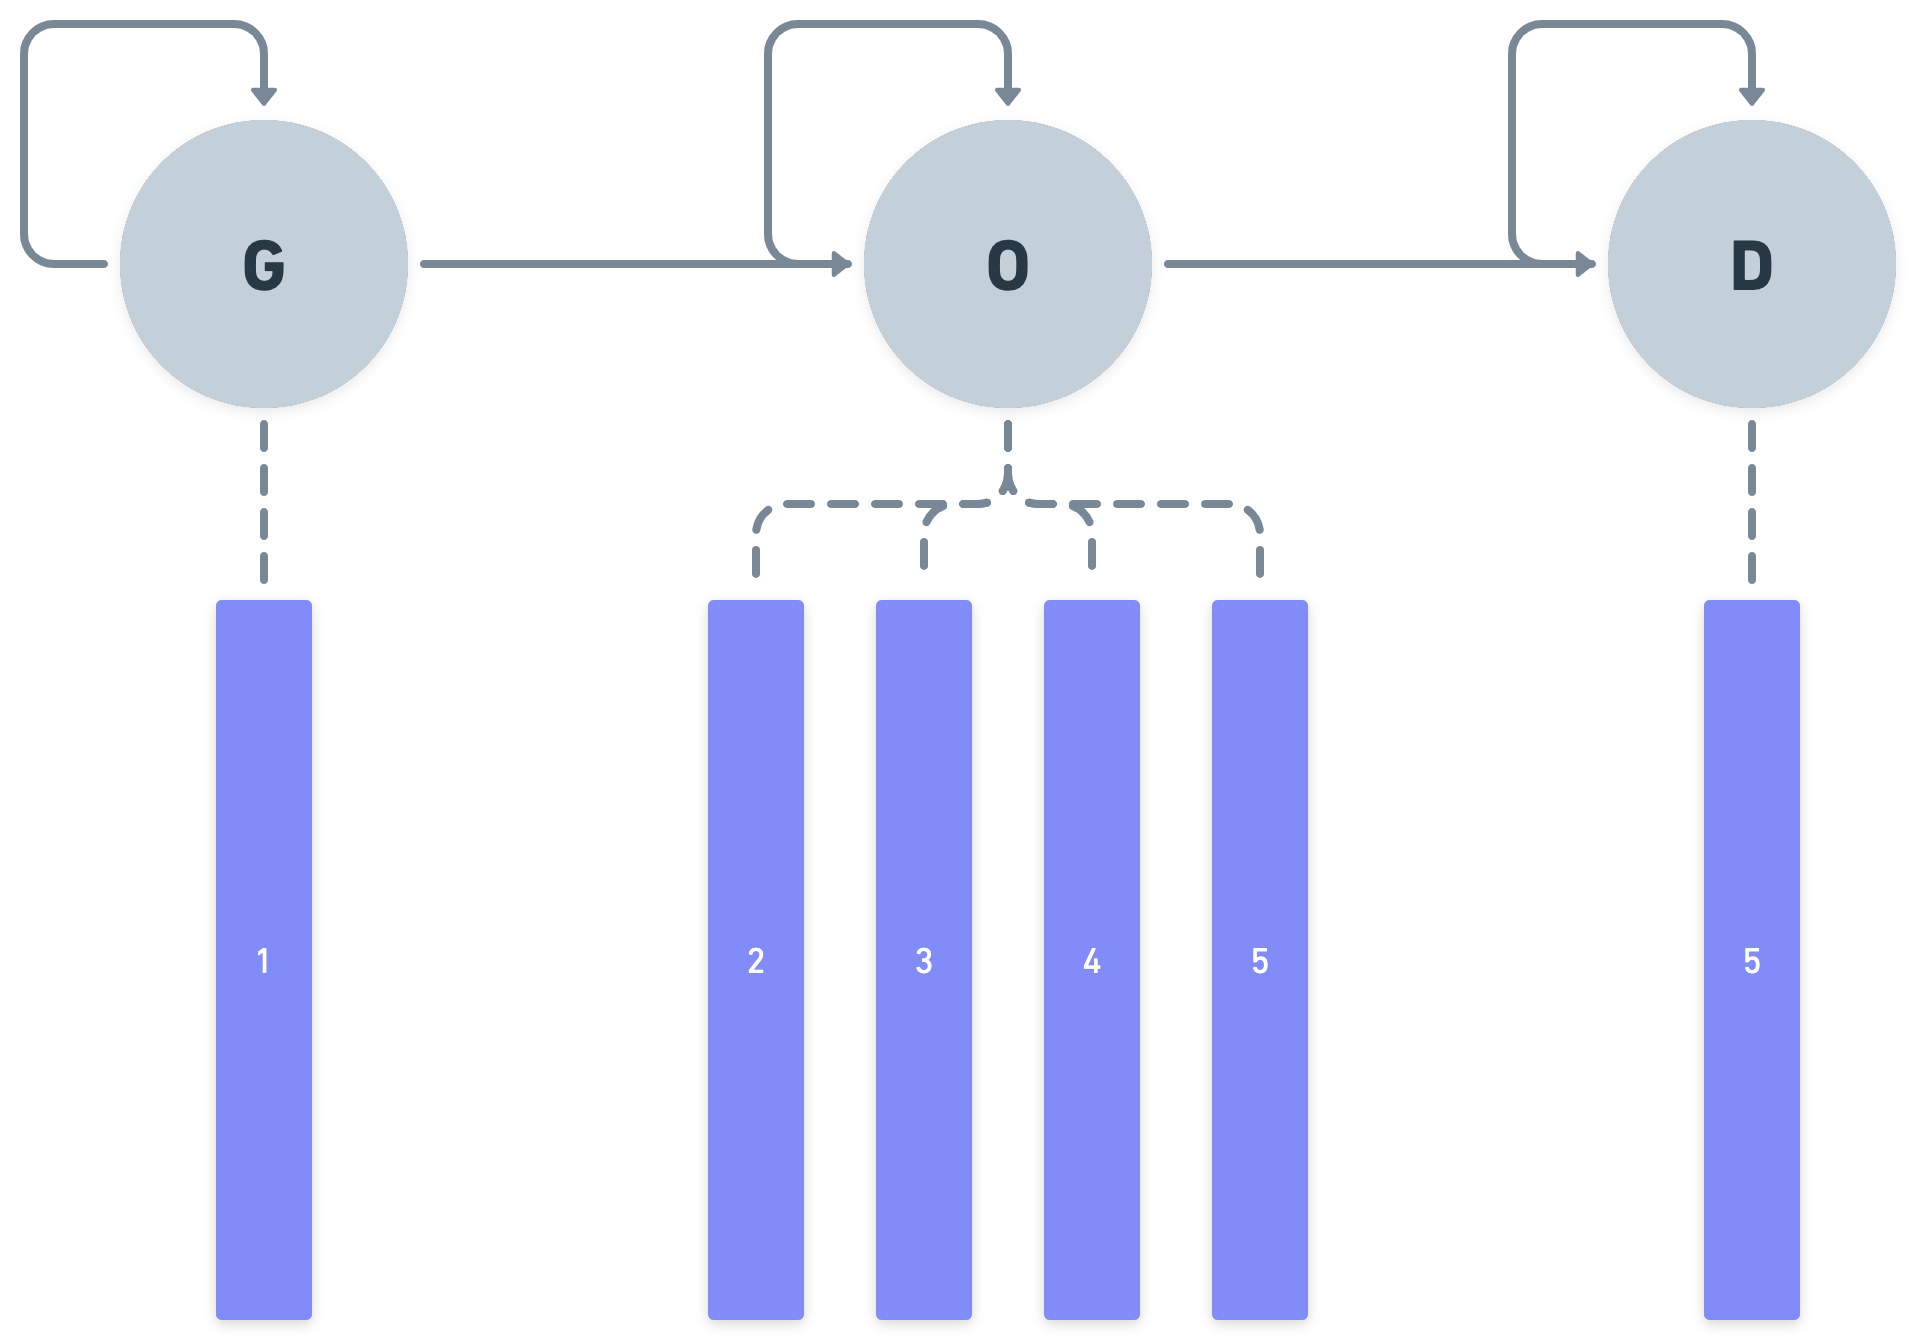
\includegraphics[width=0.65\textwidth]{figures/Q2_ALIGNMENT.png}
        \caption{HMM/DNN acoustic frame alignment}
        \label{fig:/q2_alignment}
    \end{figure}
    

    % Sub-problem 2
    \begin{subproblem}
        When training a hybrid HMM-DNN model, the cross entropy objective function is often used. Explain how this differs from the EM algorithm used to
        train standard HMM systems.
    \end{subproblem}

    \textbf{Answer}

    The EM algorithm is an iterative unsupervised optimisation algorithm, which can optimise probabilistic models such as HMMs when the training data includes
    latent veriables. It consists of two steps; the E-step which computes tge expected sufficien statistics if the latent variables given the current model
    parameters, and the M-step, which updates the model parameters based in these expected statistics. In contrast, the standard corss entropy objective function
    is a supervised technique which relies on labeled data to optimise the parameters of a neural network. This objective function then forms the loss field which
    an optimiser such as gradient descent can traverse to hopefully find a global minima.

    The main difference between these methods are the fact that the EM-algorithm learns the underlying data distribution directly from the data. Whereas the
    cross-entropy method achieves optimisation by directly using labeled data during training. The hybrid HMM/DNN model combines both these techniques such that
    the DNN model estimates the posterior probabilities using the corss-entropy objective and the HMM uses the M-step to further optimise using these posteriors.


    % Sub-problem 3
    \begin{subproblem}
        If all possible alignments are equally likely, what would be the contribution
        to the cross-entropy objective function from
        
        \begin{itemize}
            \item frame 3?
            \item frame 6?
        \end{itemize}
    \end{subproblem}

    \textbf{Answer}

    For frame 3 it is possible for either "O" or "G" being aligned to it. Therefore, the cross-entropy contributions would be the following.

    \begin{align}
        \text{"O": } E_O^3 = - ln 0.5 \approx 0.6931 \\
        \text{"G": } E_G^3 = - ln 0.5 \approx 0.6931
    \end{align}

    For frame 6 however, it will only be possible for character "G" to be aligned with it. Therefore, the cross-entropy becomes.

    \begin{align}
        \text{"G": } E_G^6 = - ln 1.0 = - 0 = \text{undefined}
    \end{align}


    % Sub-problem 4
    \begin{subproblem}
        Consider instead a character-based CTC model. List the frames that could
        be aligned to each of the CTC states.
    \end{subproblem}

    \textbf{Answer}

    In a character-based CTC model, each character is modeled by a CTC state. The CTC states are constructed such that they can generate any valid character
    sequence with any possible length, even if some characters are repeated or blank. The blank symbol $\epsilon$ is used to seperate repeated characters and
    to insert gaps between characters. In the given example of aligning the word "GOOD" to a sequence of 6 input vectors, we can construct the following CTC
    states and corresponding alignments.

    \begin{itemize}
        \item CTC state for "G": Frame 1 can be aligned to the "G" state.
        \item CTC state for "O": Frames 2 and 3 can be alignmed to the "O" state.
        \item CTC state for "D": Frames 4 and 5 can be aligned to the "D" state.
        \item Final blank state: Frame 6 can be aligned to the final blank state, which is used to indicate the end of the output sequence.
    \end{itemize}

    Note that there are multiple valid alignments, depending on the number of blanks inserted between characters and at the beginning and end of the sequence.
    The CTC algorithm computes the probability of all possible alignments and finds the most likely alignment using the forward-backward algorithm.


    % Sub-problem 5
    \begin{subproblem}
        Considering your answers above, and anything else you think is relevant,
        comment on the practical differences between cross entropy training of an
        HMM-DNN, and CTC training.
    \end{subproblem}

    \textbf{Answer}

    In terms of handling variable-length inputs and outputs, CTC training has an advantage over cross-entropy training of an HMM/DNN. With CTC, the alignment 
    between the input and output is not explicitly determined, making it more flexible in handling variable-length input and outputs. In contrast, with HMM/DNN,
    alignment is determined by the Viterbi algorithm which can be computationally expensive, and less felxible in handling variable-length inputs and outputs.

    However, one disadvantage of CTC is that it can be challenging to learn to align long sequences with many repreated characters correctly, as it requires modeling
    the distribution of repeated characters in the output sequence via the pronounciation dictrionary, which can be helpful in recognising long sequences wit repeated
    characters. Another difference is that CTC models can directly output charcter sequences, while HMM/DNN models usually output a sequence of phone or subword units,
    which need to be converted ti characters using a seperate decoding step.


    % Sub-problem 6
    \begin{subproblem}
        A Listen Attend and Spell model adopts yet another approach to alignment
        of training data. Briefly explain how alignment is performed in this model,
        and comment on the advantages and disadvantages of this approach.
    \end{subproblem}

    \textbf{Answer}

    The listen attend and spell (LAS) model is a sequence-to-sequence NN model that can be used for speech rcognition. Unlike traditional HMM-based models or CTC models,
    the LAS model does not require a pre-specified alignment between the input speech features and the output text transcription during training. Instead, the LAS model
    uses an attention mechanism to dynamically align the input speech features with the output text during training, At each time step, the attention mechanism compute a 
    context vector that is a weighted sum of the encoder outputs (i.e., the output of the NN that processes the input speech features) based on their relevance to the
    current decoding step.

    The advantages of this approach are that it allows the model to learn more flexible and accurate alignments between the input speech features and the output text, and
    it does not requrie the pre-processing step of generating forced alignments. This can be particularly useful in cases where the speech signal contains variability, such
    as different speaking rates or dialects. However, the disadvantage of this approach are that it can be more computationally intensive and may require more training data
    to learn the alignments accuratly. Additionally, the attention mechanism can sometimes focus on irrelevant parts of the input speech signal, leading to reduced accuracy.

\end{homeworkProblem}


\begin{homeworkProblem}

    % Sub-problem 1
    \begin{subproblem}
        Draw an example grammar (G) WFST that could be used to recognise the
        score announcements. You need only draw sufficent arcs to illustrate the
        concepts clearly.
    \end{subproblem}

    \textbf{Answer}

    \begin{figure}[ht]
        \centering
        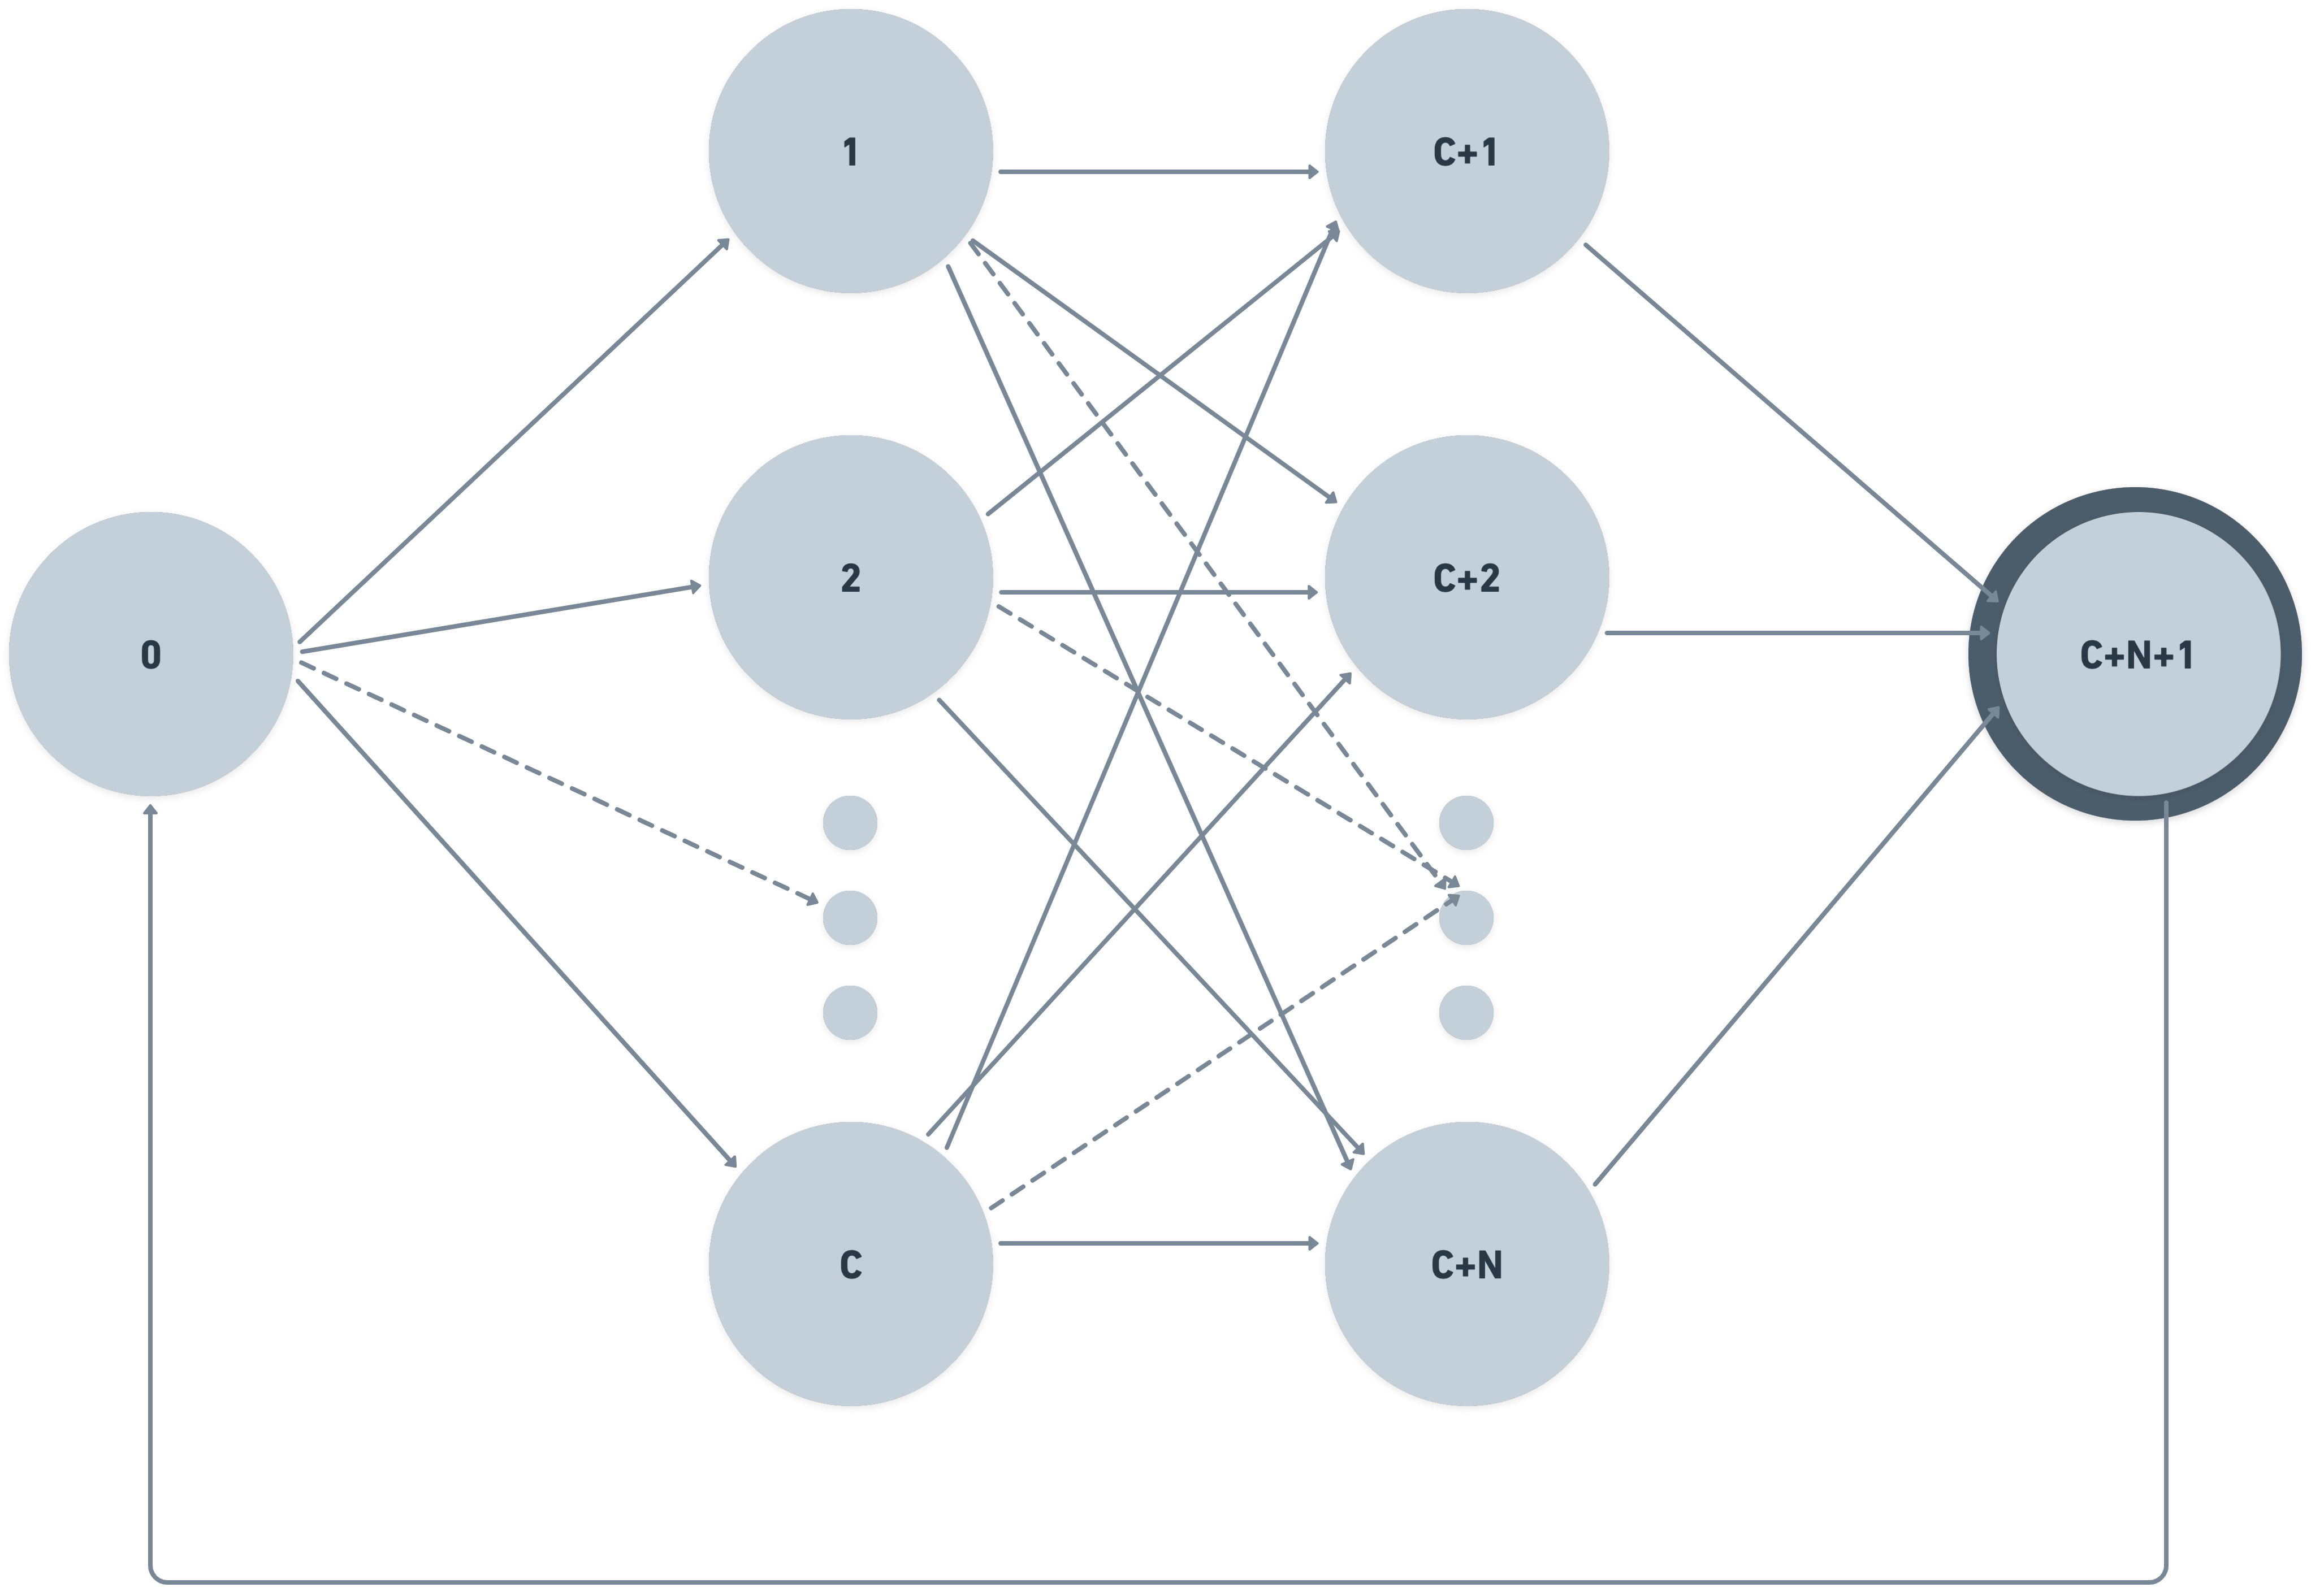
\includegraphics[width=0.65\textwidth]{figures/q3_wfst.png}
        \caption{WFST for Eurovision announcements}
        \label{fig:/q3_wfst}
    \end{figure}
    \FloatBarrier
    

    % Sub-problem 2
    \begin{subproblem}
        Draw illustrations of HMM (H) and lexicon (L) WFSTs that could be used
        in your system (you can assume that the system uses context-independent
        phones). Also illustrate the composed L ◦ G WFST, using your answer to
        part (a).
    \end{subproblem}

    \textbf{Answer}

\end{homeworkProblem}

\end{document}
